\chapter{Specifikacija programske potpore}
		
	\section{Funkcionalni zahtjevi}
			
			
			\noindent \textbf{Dionici:}
			
			\begin{packed_enum}
				
				\item Vlasnik (naručitelj)
				\item Registrirani korisnici:
							
					\begin{packed_enum}
						\item Voditelji
						\item Istraživači
						\item Tragači
					\end{packed_enum}
					
				\item Razvojni tim
				\item Administrator
				
				
			\end{packed_enum}
			
			\noindent \textbf{Aktori i njihovi funkcionalni zahtjevi:}
			
			
			\begin{packed_enum}
				
				\item  \underbar{Neregistrirani korisnik (sudionik) može:}
				
				\begin{packed_enum}
					
					\item poslati zahtjev za registraciju sa željenom ulogom za koju se prijavljuje (istraživač, voditelj postaje ili tragač na terenu)
				
				\end{packed_enum}
				
				\item \underbar{Istraživač (inicijator) može:}
				
				\begin{packed_enum}
					
					\item stvoriti nove akcije pretraživanja i praćenja
					\item poslati zahtjev voditelju za tragača s potrebnim kvalifikacijama
					\item pojedinačno zadati zadatke tragačima
						\begin{packed_enum}
							\item dati komentar za zadani zadatak
						\end{packed_enum}
					\item pristupiti interaktivnoj karti s informacijama o poziciji tragača, životinja i postaja
						\begin{packed_enum}
							\item ostaviti komentar za ostale sudionike
						\end{packed_enum} 
					\item odabrati prikaz na karti (povijesne pozicije životinja, filtrirano po vrsti, filtrirano po jedinki, trenutne pozicije životinja; povijesne pozicije tragača, filitrirano po tipu prijevoza, filtrirano pojedinačno po tragaču, trenutne pozicije tragača)
					
				\end{packed_enum}	
				
				\item \underbar{Voditelj postaje (inicijator) može:}
				
				\begin{packed_enum}
					
					\item definirati tragače njegove postaje
						\begin{packed_enum}
							\item definirati način na koji su osposobljeni izvoditi pretraživanje
						\end{packed_enum}
					\item odabrati konkretne tragače za pojedinu akciju
					
				\end{packed_enum}
			
				\item \underbar{Tragač na terenu (inicijator) može:}
					
					\begin{packed_enum}
						\item obavljati zadatke na različite načine (pješke, dronom, automobilom, 
						cross motorom, brodom, helikopterom)
						\item ostaviti komentar o životinji tijekom akcije
						\item maknuti se s akcije završetkom potrebnih zadataka
						\item pristupiti interaktivnoj karti s informacijama o zadacima, poziciji tragača te trenutnim pozicijama životinja
							\begin{packed_enum}
								\item ostaviti komentar za ostale sudionike
							\end{packed_enum}
					\end{packed_enum}
					
				\item \underbar{Administrator (inicijator) može:}
				
					\begin{packed_enum}
						\item vidjeti popis registriranih korisnika i njihove podatke
						\begin{packed_enum}
							\item mijenjati prava i podatke registriranih korisnika
						\end{packed_enum}
						\item potvrditi istraživača i voditelja postaje
					\end{packed_enum}
					
				\item \underbar{Baza podataka (sudionik):}
				
					\begin{packed_enum}
						\item pohranjuje sve podatke o korisnicima i njihovim ovlastima
						\item pohranjuje sve podatke o postajama i njihovim lokacijama
						\item pohranjuje sve podatke o životinjama i njihovim lokacijama
					\end{packed_enum}
			\end{packed_enum}
			
			
			\eject 
			
			
				
			\subsection{Obrasci uporabe}
				
					
					\noindent \underbar{\textbf{UC1 - Registracija}}
					\begin{packed_item}
						
						\item \textbf{Glavni sudionik: } Neregistrirani korisnik
						\item  \textbf{Cilj:} Izrada korisničkog računa za pristup sustavu
						\item  \textbf{Sudionici:} Baza podataka
						\item  \textbf{Preduvjet:} -
						\item  \textbf{Opis osnovnog tijeka:}
						
						\item[] \begin{packed_enum}
							
							\item Odabir opcije registracija
							\item Odabir uloge
							\item Unos osobnih podataka (korisničko ime, fotografija, lozinka, ime, prezime i email adresa)
							\item Slanje zahtjeva za registraciju
							\item Potvrđivanje registracije preko email adrese
							
						
								\end{packed_enum}
								
						\item  \textbf{Opis mogućih odstupanja:}
						
						\item[] \begin{packed_item}
							
							\item[3.a] Zauzeto korisničko ime
							\begin{packed_enum}
								
								\item Sustav obavještava korisnika da je potrebno upotrijebiti drugo korisničko ime
								
								\end{packed_enum}
							
							\item[3.b] Krivi format lozinke \begin{packed_enum}
								
								\item Sustav obavještava korisnika o uvjetu koji nije zadovoljen da bi lozinka bila ispravna
								
								\end{packed_enum}
							
							\item[3.c] Nepotpuna prijava \begin{packed_enum}
								
								\item Sustav obavještava korisnika o podacima koji mu nedostaju za uspješnu registraciju
								
								\end{packed_enum}
							
							\item[5.a] Nije potvrđena registracije preko email adrese \begin{packed_enum}
								
								\item Sustav obavještava korisnika da mora potvrditi registraciju preko email adrese
								
							\end{packed_enum}
							
						\end{packed_item}
						
					\end{packed_item}
					
					
					\noindent \underbar{\textbf{UC2 - Potvrda registracije od strane administratora}}
					\begin{packed_item}
						
						\item \textbf{Glavni sudionik: }Administrator
						\item  \textbf{Cilj:} Potvrda registracije istraživača i voditelja
						\item  \textbf{Sudionici:} Baza podataka
						\item  \textbf{Preduvjet:} Istraživač ili voditelj je poslao zahtjev za registraciju i potvrdio registraciju putem mail-a.
						\item  \textbf{Opis osnovnog tijeka:}
						
						\item[] \begin{packed_enum}
							
							\item Odabir opcije potvrđivanja registracije istraživača i voditelja
							
						\end{packed_enum}
						
						
					\end{packed_item}
					
					
					\noindent \underbar{\textbf{UC3 - Prijava u sustav}}
					\begin{packed_item}
						
						\item \textbf{Glavni sudionik: }Korisnik
						\item  \textbf{Cilj:} Korištenje aplikacije
						\item  \textbf{Sudionici:} Baza podataka
						\item  \textbf{Preduvjet:} Potvrđena registracija
						\item  \textbf{Opis osnovnog tijeka:}
						
						\item[] \begin{packed_enum}
							
							\item Odabir opcije prijava
							\item Unos podataka (korisničko ime i lozinka)
							\item Otvaranje aplikacije
					
							
						\end{packed_enum}
						
						\item  \textbf{Opis mogućih odstupanja:}
						
						\item[] \begin{packed_item}
							
							\item[2.a] Unos pogrešnog korisničkog imena ili lozinke
							\item[] \begin{packed_enum}
								
								\item Sustav obavještava korisnika da je unio pogrešno korisničko ime ili lozinku te mu dozvoljava novi pokušaj
								
								\end{packed_enum}
							
						\end{packed_item}
						
					\end{packed_item}
					
					\noindent \underbar{\textbf{UC4 - Uređivanje osobnih podataka}}
					\begin{packed_item}
						
						\item \textbf{Glavni sudionik: }Korisnik
						\item  \textbf{Cilj:} Promijenjeni osobni podaci
						\item  \textbf{Sudionici:} Baza podataka
						\item  \textbf{Preduvjet:} Korisnik je prijavljen u sustav
						\item  \textbf{Opis osnovnog tijeka:}
						
						\item[] \begin{packed_enum}
							
							\item Odabir opcije "Osobni podaci"
							\item Odabir opcije "Uredi"
							\item Promjena željenih podataka
							\item Odabir opcije "Spremi"
							\item Baza podataka se ažurira
							
						\end{packed_enum}
						
						\item  \textbf{Opis mogućih odstupanja:}
						
						\item[] \begin{packed_item}
							
							\item[3.a] Unos zauzetog korisničkog imena
							\item[] \begin{packed_enum}
								
								\item Sustav obavještava korisnika da je potrebno upotrijebiti drugu korisničko ime
								
							\end{packed_enum}
							
						\end{packed_item}
						
						\item[] \begin{packed_item}
							
							\item[3.b] Korisnik unosi krivi format lozinke
							\item[] \begin{packed_enum}
								
								\item Sustav obavještava korisnika o uvjetu koji nije zadovoljen da bi lozinka bila ispravna
								
							\end{packed_enum}
							
						\end{packed_item}
						
						\item[] \begin{packed_item}
							
							\item[4.a]Korisnik ne odabire opciju "Spremi"
							\item[] \begin{packed_enum}
								
								\item Sustav obavještava korisnika da nije spremio podatke 
								
							\end{packed_enum}
							
						\end{packed_item}
					\end{packed_item}
					
					\noindent \underbar{\textbf{UC5 - Pregled registriranih korisnika}}
					\begin{packed_item}
						
						\item \textbf{Glavni sudionik: }Administrator
						\item  \textbf{Cilj:} Pregled registriranih korisnika
						\item  \textbf{Sudionici:} Baza podataka
						\item  \textbf{Preduvjet:} Postoje registrirani korisnici
						\item  \textbf{Opis osnovnog tijeka:}
						
						\item[] \begin{packed_enum}
							
							\item Odabir opcije pregleda registriranih korisnika
							\item Pregled podataka
							
						\end{packed_enum}
						
						
					\end{packed_item}
					
					\noindent\underbar{\textbf{UC6 - Upravljanje registriranim korisnicima}}
					\begin{packed_item}
						
						\item \textbf{Glavni sudionik: }Administrator
						\item  \textbf{Cilj:} Upravljanje registriranim korisnicima
						\item  \textbf{Sudionici:} Baza podataka
						\item  \textbf{Preduvjet:} Postoje registrirani korisnici
						\item  \textbf{Opis osnovnog tijeka:}
						
						\item[] \begin{packed_enum}
							
							\item Odabir opcije mijenjanja prava i osobnih podataka pojedinog korisnika
							\item Odabir opcije spremanja promjene
							\item Baza podataka se ažurira
							
						\end{packed_enum}
						
						\item  \textbf{Opis mogućih odstupanja:}
						
						\item[] \begin{packed_item}
							
							\item[2.a] Administrator ne odabire opciju spremanja promjena
							\item[] \begin{packed_enum}
								
								\item Sustav obavještava korisnika da nije spremio podatke 
								
							\end{packed_enum}
							
						\end{packed_item}
						
					\end{packed_item}
					
					\noindent \underbar{\textbf{UC7 - Odabir  postaje i tragača}}
					\begin{packed_item}
						
						\item \textbf{Glavni sudionik: }Voditelj
						\item  \textbf{Cilj:} Voditelj ima dodijeljenu postaju i tragače kojima upravlja
						\item  \textbf{Sudionici:} Baza podataka
						\item  \textbf{Preduvjet:} Prijavljen kao voditelj
						\item  \textbf{Opis osnovnog tijeka:}
						
						\item[] \begin{packed_enum}
							
							\item Voditelj unosi naziv postaje koje će pokrivati
							\item Voditelj odabire tragače koji su dio njegove postaje
							
							\end{packed_enum}
						\item  \textbf{Opis mogućih odstupanja:}
						
						\item[] \begin{packed_item}
							
							\item[2.a] Voditelj odabire već zauzetu postaju
							\item[] \begin{packed_enum}
								
								\item Sustav obavještava voditelja da ta postaja već postoji
								
							\end{packed_enum}
							
						\end{packed_item}
						
						
					\end{packed_item}
					
					\noindent \underbar{\textbf{UC8 - Definiranje metode pretraživanja tragača}}
					\begin{packed_item}
						
						\item \textbf{Glavni sudionik: }Voditelj
						\item  \textbf{Cilj:} Tragač ima definirane metode pretraživanja
						\item  \textbf{Sudionici:} Baza podataka
						\item  \textbf{Preduvjet:} Voditelj ima dodijeljenu postaju i tragače kojima upravlja
						\item  \textbf{Opis osnovnog tijeka:}
						
						\item[] \begin{packed_enum}
							
							\item Voditelj odabire tragača
							\item Voditelj definira načine na koje je odabrani tragač osposobljen pretraživati (pješke, dronom, automobilom, cross motorm, brodom ili helikopterom)
							
							
						\end{packed_enum}
						
						
					\end{packed_item}
					
					\noindent \underbar{\textbf{UC9 - Praćenje životinja}}
					\begin{packed_item}
						
						\item \textbf{Glavni sudionik:} Gps uređaj
						\item  \textbf{Cilj:} Praćenje životinja
						\item  \textbf{Sudionici:} Baza podataka
						\item  \textbf{Preduvjet:} Postavljen gps uređaj na životinji
						\item  \textbf{Opis osnovnog tijeka:}
						
						\item[] \begin{packed_enum}
							
							\item Gps uređaj aplikaciji odašilje svoju poziciju
							\item U bazu podataka se zapisuju podaci o životinji
							
						\end{packed_enum}
						
						\item  \textbf{Opis mogućih odstupanja:}
						
						\item[] \begin{packed_item}
							
							\item[1.a] Gps uređaj ne radi
							\item[] \begin{packed_enum}
								
								\item Sustav obavještava korisnike da je gps uređaj prestao raditi
								
							\end{packed_enum}
							
						\end{packed_item}
						
					\end{packed_item}
					
					\noindent \underbar{\textbf{UC10 - Stvaranje akcije pretraživanja i praćenja}}
					\begin{packed_item}
						
						\item \textbf{Glavni sudionik: }Istraživač
						\item  \textbf{Cilj:} Stvoriti akciju pretraživanja i praćenja
						\item  \textbf{Sudionici:} Baza podataka
						\item  \textbf{Opis osnovnog tijeka:}
						
						\item[] \begin{packed_enum}
							
							\item Istraživač odabire opciju stvaranja nove akcije
							\item Istraživač odabire postaju, broj tragača te potrebne kvalifikacije za akciju 
							\item Istraživač šalje zahtjev za tragačima voditelju postaje
							
							
						\end{packed_enum}
							
						
					\end{packed_item}
					
						\noindent \underbar{\textbf{UC11 - Odabir tragača za akciju}}
					\begin{packed_item}
						
						\item \textbf{Glavni sudionik: }Voditelj
						\item  \textbf{Cilj:} Odabrati tragače za akciju pretraživanja i praćenja
						\item  \textbf{Sudionici:} Baza podataka
						\item  \textbf{Preduvjet:} Voditelj posjeduje tragače koji nisu niti na jednoj akciji
						\item  \textbf{Opis osnovnog tijeka:}
						
						\item[] \begin{packed_enum}
							
							\item Voditelj postaje prima zahtjev od istraživača za određenim brojem tragača s određenim kvalifikacijama
							\item  Voditelj postaje odabire tragače za akciju
							\item Voditelj postaje šalje popis odabranih tragača istraživaču
							
						\end{packed_enum}
						
						\item  \textbf{Opis mogućih odstupanja:}
						
						\item[] \begin{packed_item}
							
							\item[2.a] Voditelj postaje nema dovoljan broj tragača s potrebnim kvalifikacijama
							\item[] \begin{packed_enum}
								
								\item Voditelj obavještava istraživača kako nema dovoljan broja tragača te mu dodjeljuje one koje ima
								
							\end{packed_enum}
							
						\end{packed_item}
						
					\end{packed_item}
					
					
					
					\noindent \underbar{\textbf{UC12 - Stvaranje zadataka}}
					\begin{packed_item}
						
						\item \textbf{Glavni sudionik: }Istraživač
						\item  \textbf{Cilj:} Stvaranje zadataka na pojedinoj akciji
						\item  \textbf{Sudionici:} Baza podataka
						\item  \textbf{Preduvjet:} Istraživač je prijavljen
						\item  \textbf{Opis osnovnog tijeka:}
						
						\item[] \begin{packed_enum}
							
							\item Odabir određenog tragača
							\item Odabir opcije dodavanja novog zadatka odabranom tragaču
							\item Odabir zadatka (prolazak određenom rutom i dolazak do određene lokacije, postavljanje
							kamere ili uređaja za praćenje)
							\item Istraživač potvrđuje unesene podatke i time dodijeljuje zadatak tragaču
							\item Spremanje podataka u bazu podataka
						\end{packed_enum}
						
						\item  \textbf{Opis mogućih odstupanja:}
						
						\item[] \begin{packed_item}
							
							
							\item[4.a] Istraživač ne potvrđuje unesene podatke
							\item[] \begin{packed_enum}
								
								\item Sustav obavještava korisnika da nije potvrdio podatke prije izlaska iz prozora
								
								\end{packed_enum}
							
						\end{packed_item}
						
					\end{packed_item}
					
					\noindent \underbar{\textbf{UC13 - Ostavljanje komentara za tragače}}
					\begin{packed_item}
						
						\item \textbf{Glavni sudionik:} Istraživač
						\item  \textbf{Cilj:} Ostaviti komentare za akciju tragačima 
						\item  \textbf{Sudionici:} Baza podataka
						\item  \textbf{Preduvjet:} Zadaci za tragače su stvoreni
						\item  \textbf{Opis osnovnog tijeka:}
						
						\item[] \begin{packed_enum}
							
							\item Istraživaču se nudi opcija dodavanja komentara na zadatak
							\item Istraživač unosi i sprema komentar
							
						\end{packed_enum}
						
						\item  \textbf{Opis mogućih odstupanja:}
						
						\item[] \begin{packed_item}
							
							\item[4.a]Korisnik ne odabire opciju "Spremi"
						\item[] \begin{packed_enum}
							
							\item Sustav obavještava korisnika da nije spremio komentar
							
						\end{packed_enum}
							
						\end{packed_item}
						
					\end{packed_item}
					
					\noindent \underbar{\textbf{UC14 - Prikaz životinja na karti istraživača}}
					\begin{packed_item}
						
						\item \textbf{Glavni sudionik: }Istraživač
						\item  \textbf{Cilj:} Prikaz životinja na karti
						\item  \textbf{Sudionici:} Baza podataka
						\item  \textbf{Preduvjet:} Istraživač je prijavljen i izradio je akciju
						\item  \textbf{Opis osnovnog tijeka:}
						
						\item[] \begin{packed_enum}
							
							\item Odabir prikaza karte
							\item Odabir prikaza životinja 
							
							\item Odabir informacija koje će se prikazivati na karti (povijesne pozicije svih praćenih životinja filtrirano po vrsti ili pojedinačno po jedinki, trenutne pozicije praćenih životinja)
							\item Odabir opcije generiranja karte
							\item Sustav generira kartu na temelju odabranih podataka (za informacije o povijesnim pozicijama generira se toplinska karta)
							
						\end{packed_enum}
						\item  \textbf{Opis mogućih odstupanja:}
						
						\item[] \begin{packed_item}
							
							\item[5.a]Korisnik nije odabrao sve potrebne informacije 
							\item[] \begin{packed_enum}
								
								\item Sustav obavještava korisnika da nije odabrao sve potrebne informacije
								
							\end{packed_enum}
							
						\end{packed_item}
					\end{packed_item}
						
						
						
				\noindent \underbar{\textbf{UC15 - Prikaz tragača na karti istraživača}}
				\begin{packed_item}
					
					\item \textbf{Glavni sudionik: }Istraživač
					\item  \textbf{Cilj:} Prikaz tragača na karti
					\item  \textbf{Sudionici:} Baza podataka
					\item  \textbf{Preduvjet:} Istraživač je prijavljen i izradio je akciju
					\item  \textbf{Opis osnovnog tijeka:}
					
					\item[] \begin{packed_enum}
						
						\item Odabir prikaza karte
						\item Odabir prikaza tragača
						\item Odabir informacija koje će se prikazivati na karti (povijesne pozicije svih tragača na nekoj akciji, filtrirano po tipu prijevoza ili pojedinačno po tragaču te trenutne pozicije tragača aktivnih na akciji)
						\item Odabir opcije generiranja karte
						\item Sustav generira kartu na temelju odabranih podataka (za informacije o povijesnim pozicijama generira se toplinska karta)
						
					\end{packed_enum}
					
					\item  \textbf{Opis mogućih odstupanja:}
					
					\item[] \begin{packed_item}
						
						\item[5.a]Karta se ne generira 
						\item[] \begin{packed_enum}
							
							\item Sustav obavještava korisnika da nije odabrao sve potrebne informacije
							
						\end{packed_enum}
						
					\end{packed_item}
				\end{packed_item}
				
	
			
			
				
				\noindent \underbar{\textbf{UC16 - Prikaz karte za tragača}}
				\begin{packed_item}
					
					\item \textbf{Glavni sudionik:}Tragač
					\item  \textbf{Cilj:} Prikaz karte za tragača s pripadajućim zadacima te označavanje odrađenih zadataka na akciji
					\item  \textbf{Sudionici:} Baza podataka
					\item  \textbf{Preduvjet:} Tragač je prijavljen i sudjeluje u određenoj akciji
					\item  \textbf{Opis osnovnog tijeka:}
					
					\item[] \begin{packed_enum}
						
						\item Odabir određene akcije
						\item Odabir prikaza karte za odabranu akciju
						\item Odabir prikaza popisa zadataka, trenutne pozicije ostalih tragača ili trenutne pozicije praćenih životinja za određenu akciju
						\item Tragač može pojedini zadatak označiti odrađenim
						\item Tragač potvrđuje unesene podatke
						\item Spremanje podataka u bazu podataka
					\end{packed_enum}
					
					\item  \textbf{Opis mogućih odstupanja:}
					
					\item[] \begin{packed_item}
						
						
						\item[5.a] Tragač ne potvrđuje unesene podatke
						\item[] \begin{packed_enum}
							
							\item Sustav obavještava korisnika da nije potvrdio podatke prije izlaska iz prozora
							
						\end{packed_enum}
						
					\end{packed_item}
					
				\end{packed_item}
				
				\noindent \underbar{\textbf{UC17 - Ostavljanje komentara o životinji}}
				\begin{packed_item}
					
					\item \textbf{Glavni sudionik:}Tragač/Istraživač
					\item  \textbf{Cilj:} Komentar za životinju 
					\item  \textbf{Sudionici:} Baza podataka
					\item  \textbf{Preduvjet:} Tragač je sudjelovao u akciji
					\item  \textbf{Opis osnovnog tijeka:}
					
					\item[] \begin{packed_enum}
					 
						\item Pri prikazu karte	nudi se opcija "Komentiraj"
					\item Pisanje komentara za praćenu životinju
						\item  Spremanje komentara
					\end{packed_enum}
					
						\item  \textbf{Opis mogućih odstupanja:}
					
					\item[] \begin{packed_item}
						
						\item[4.a]Korisnik ne odabire opciju "Spremi"
						\item[] \begin{packed_enum}
							
							\item Sustav obavještava korisnika da nije spremio komentar
							
						\end{packed_enum}
						
					\end{packed_item}
					
				\end{packed_item}
				
				
				
				\noindent \underbar{\textbf{UC18 - Napuštanje akciju}}
				\begin{packed_item}
					
					\item \textbf{Glavni sudionik: }Tragač
					\item  \textbf{Cilj:} Tragač više ne sudjeluje u akciji
					\item  \textbf{Sudionici:} Baza podataka
					\item  \textbf{Preduvjet:} Tragač je ispunio sve dodijeljene zadatke
					\item  \textbf{Opis osnovnog tijeka:}
					
					\item[] \begin{packed_enum}
						
						\item Tragač odabire određenu akciju
						\item Tragač odabire opciju za napuštanje akcije

					\end{packed_enum}
					
					\item  \textbf{Opis mogućih odstupanja:}
					
					\item[] \begin{packed_item}
						
						\item[1.a] Tragač pokušava napustiti akciju, a nije izvršio sve zadatke
						\item[] \begin{packed_enum}
							
							\item Sustav obavještava tragača da nije ispunio sve zadatke te mu ne dopušta napustiti akciju
							
						\end{packed_enum}
						
					\end{packed_item}
					
				\end{packed_item}
				
				\noindent \underbar{\textbf{UC1 - Ocjena i komentiranje završene akcije}}
				\begin{packed_item}
					
					\item \textbf{Glavni sudionik: }Tragač
					\item  \textbf{Cilj:} Tragač ostavlja ocjenu i komentar
					\item  \textbf{Sudionici:} Baza podataka
					\item  \textbf{Preduvjet:} Tragač je završio akciju
					\item  \textbf{Opis osnovnog tijeka:}
					
					\item[] \begin{packed_enum}
						
						\item Nakon završetka akcije, tragaču se nudi opcija "Ocijeni"
						\item Tragač odabire ocjenu za odrađenu akciju
						\item Tragaču se nudi opcija "Komentiraj"
						\item Tragač piše komentar na akciju
						\item Tragač sprema ocjenu i komentar
						
					\end{packed_enum}
					
						\item  \textbf{Opis mogućih odstupanja:}
					
					\item[] \begin{packed_item}
						
						\item[4.a]Korisnik ne odabire opciju "Spremi"
						\item[] \begin{packed_enum}
							
							\item Sustav obavještava korisnika da nije spremio komentar
							
						\end{packed_enum}
						
					\end{packed_item}
				\end{packed_item}
				
				
				\noindent \underbar{\textbf{UC20 - Blježenje staza i kretanja tragača}}
				\begin{packed_item}
					
					\item \textbf{Glavni sudionik:}Tragač
					\item  \textbf{Cilj:} Bilježenje staza i kretanja tragača
					\item  \textbf{Sudionici:} Baza podataka
					\item  \textbf{Preduvjet:} Tragač je prijavljen i koristi gps uređaj
					\item  \textbf{Opis osnovnog tijeka:}
					
					\item[] \begin{packed_enum}
						
						\item Tragač ima uključen gps uređaj prilikom obavljanja zadatka
						\item Gps uređaj odašilje svoju poziciju
						\item Tragač ima opciju unijeti način kojim se kretao
						\item Tragač potvrđuje unešeni način
						
					\end{packed_enum}
					
					\item  \textbf{Opis mogućih odstupanja:}
					
					\item[] \begin{packed_item}
						
						\item[1.a] Tragač nije uključio gps uređaj
						\item[] \begin{packed_enum}
							
							\item Sustav obavještava tragača da nije uključen gps uređaj
							
						\end{packed_enum}
						
						\item[2.a] Gps uređaj ne radi
						\item[] \begin{packed_enum}
							
							\item Sustav obavještava tragača da gps uređaj ne radi
							
						\end{packed_enum}
						
						\item[3.a] Tragač ne potvrđuje unesene podatke
						\item[] \begin{packed_enum}
							
							\item Sustav obavještava korisnika da nije potvrdio podatke prije izlaska iz prozora
							
						\end{packed_enum}
						
					\end{packed_item}
					
				\end{packed_item}
					
					
					
				\subsubsection{Dijagrami obrazaca uporabe}
						
				
				\begin{figure}[H]
					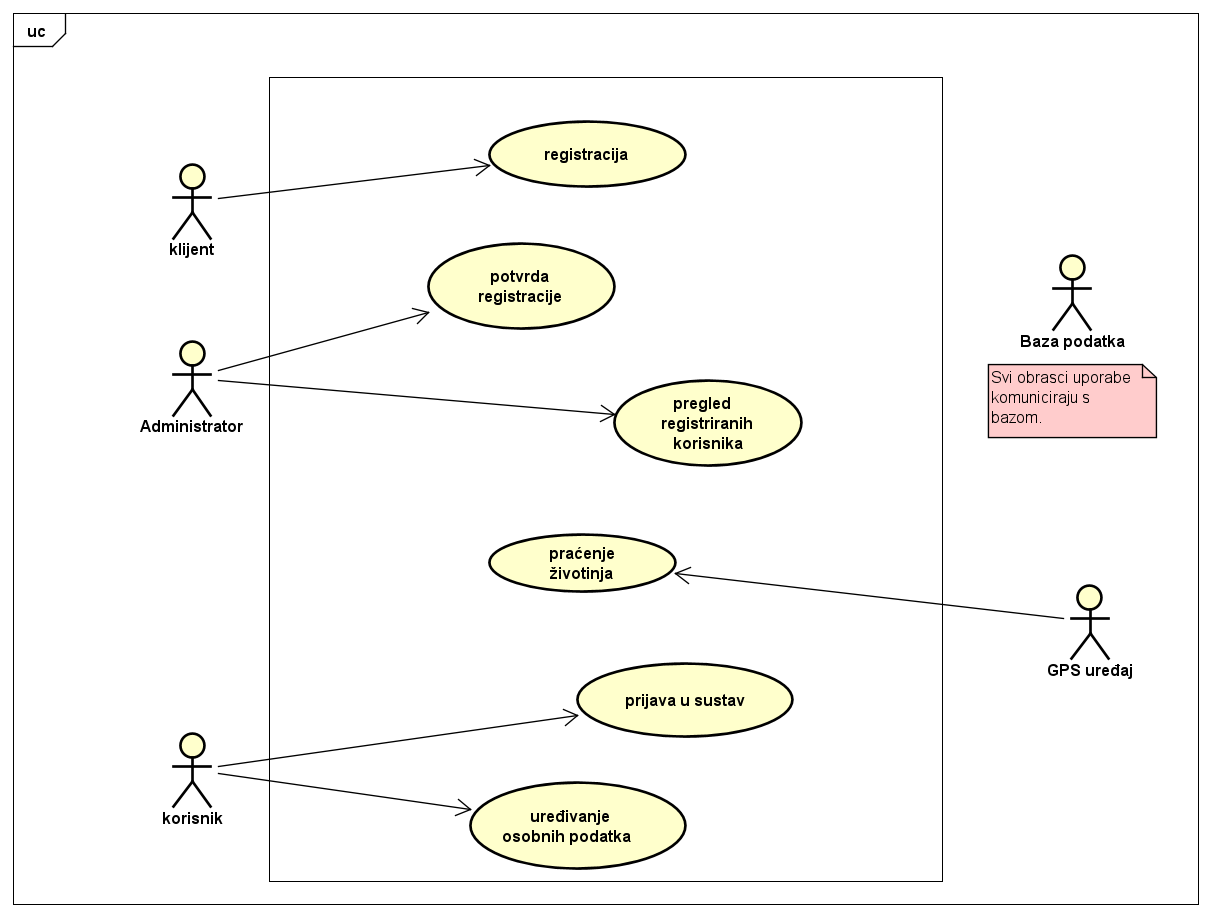
\includegraphics[scale=0.5]{slike/dijagram1.PNG} %veličina u odnosu na širinu linije
					\centering
					\caption{Dijagram obrasca uporabe, funkcionalnost administratora, klijenta, korisnika i GPS uređaja}
					\label{fig:dijagram1} %label mora biti drugaciji za svaku sliku
				\end{figure}
				
				\begin{figure}[H]
					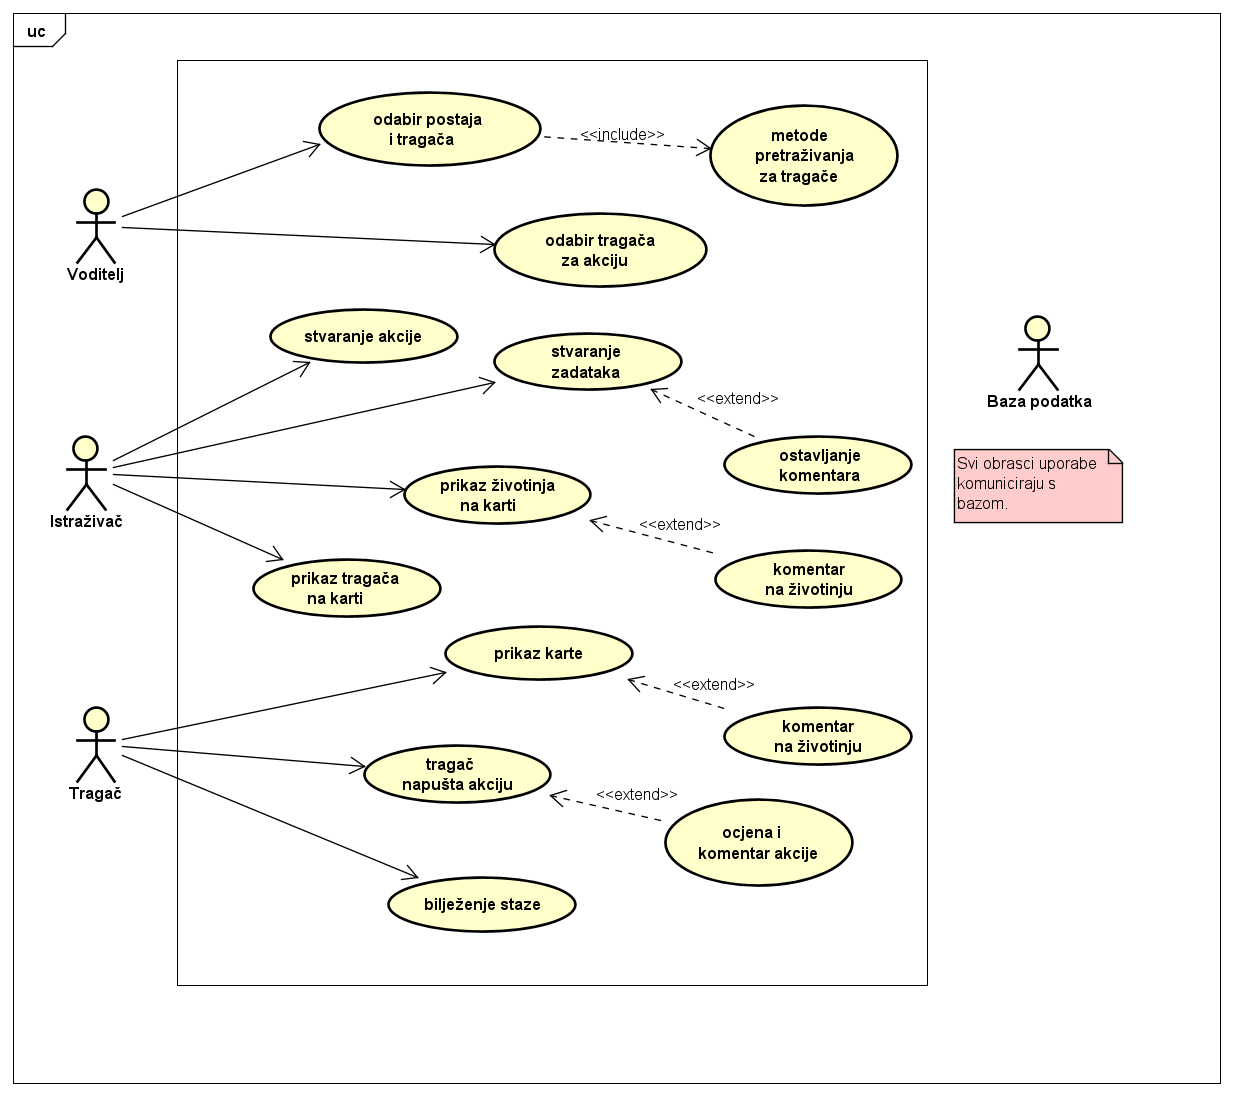
\includegraphics[scale=0.5]{slike/dijagram2.PNG} %veličina u odnosu na širinu linije
					\centering
					\caption{Dijagram obrasca uporabe, funkcionalnost voditelja, istraživača i tragača}
					\label{fig:dijagram2} %label mora biti drugaciji za svaku sliku
				\end{figure}
				
			\subsection{Sekvencijski dijagrami}
				
				\noindent \textbf{Obrazac uporabe UC6 - Voditelj odabire svoje postaje i tragače}\\
				
				\noindent Voditelj šalje zahtjev za prikaz stranice za odabir postaje i tragača. Poslužitelj prima zahtjev te iz baze podataka dohvaća dostupne tragače i prikazuje traženu stranicu voditelju. Voditelj odabire željenu postaju i tragače koji će biti vezani za tu postaju te potvrđuje svoj odabir. Poslužitelj prima potvrdu i sprema podatke o voditelju, postaji i tragačima u bazu podataka. Baza vraća potvrdu, a poslužitelj voditelju prikazuje stranicu s informacijama o njegovoj postaji.
				
				\begin{figure}[H]
					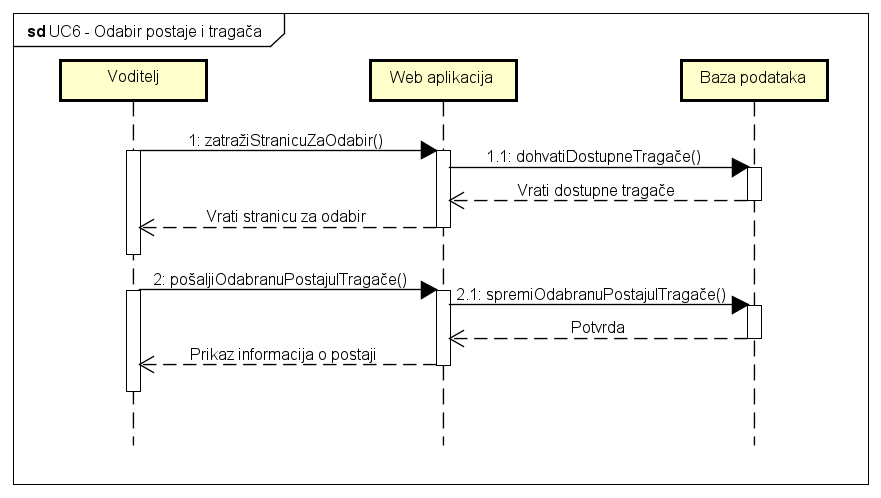
\includegraphics[scale=0.7]{slike/UC6_sekv.PNG} %veličina slike u odnosu na originalnu datoteku i pozicija slike
					\centering
					\caption{Sekvencijski dijagram - UC6}
					\label{fig:promjene}
				\end{figure}
				\eject
				
				\noindent \textbf{Obrazac uporabe UC7 - Voditelj definira metode pretraživanja igrača}\\
				
				\noindent Voditelj šalje zahtjev za prikaz stranice s popisom tragača i njihovih trenutnih metoda pretraživanja. Poslužitelj prima zahtjev te iz baze podataka dohvaća odabrane tragače i njihove metode pretraživanja nakon čega prikazuje voditelju stranicu za promjenu metoda pretraživanja. Ako tragač nema odabranu metodu, nedostupan je za akcije i voditelju je to naznačeno posebnom porukom te je potrebno odabrati jednu od metoda. Voditelj odabire metode pretraživanja svim željenim tragačima te šalje nove podatke poslužitelju. Postlužitelj te podatke šalje u bazu podataka koja vraća poruku potvrde, a poslužitelj voditelju prikazuje stranicu s informacijama o njegovoj postaji.
				
				\begin{figure}[H]
					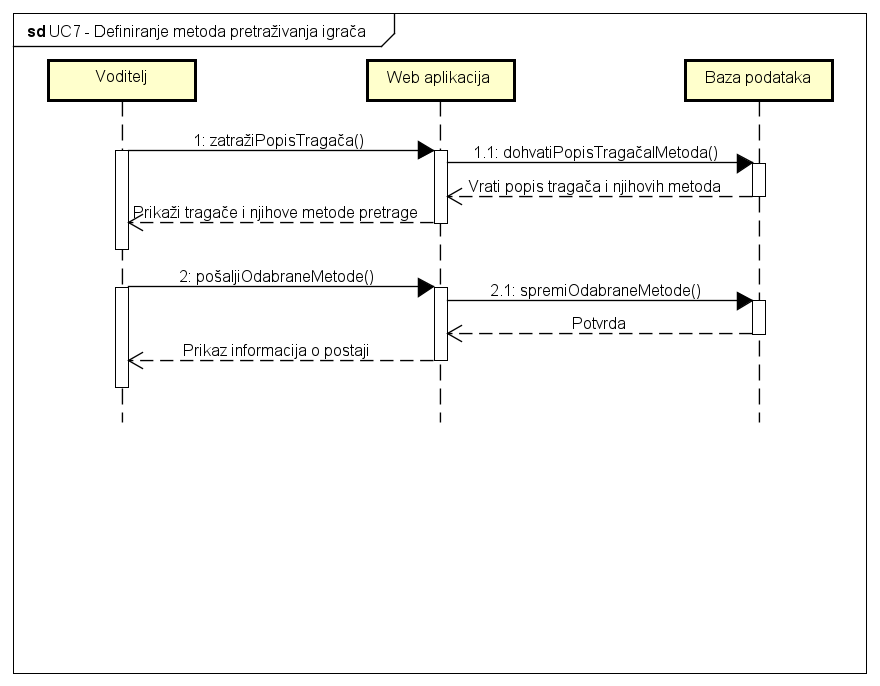
\includegraphics[scale=0.7]{slike/UC7_sekv.PNG} %veličina slike u odnosu na originalnu datoteku i pozicija slike
					\centering
					\caption{Sekvencijski dijagram - UC7}
					\label{fig:promjene}
				\end{figure}
				\eject
				
				\noindent \textbf{Obrazac uporabe UC11 - Stvaranje zadataka}\\
				
				\noindent Istraživač šalje zahtjev za prikazom stranice za dodjelu zadataka. Poslužitelj dohvaća dostupne tragače iz baze podataka te ih prikazuje istraživaču. Istraživač dodjeljuje zadatke za svakog tragača posebno (prolazak određenom rutom, dolazak do određene lokacije, postavljanje kamere ili uređaja za praćenje) upisom u formu pojedinačnog tragača. Nakon dodjele zadataka istraživač šalje zahtjev za spremanjem podataka. Poslužitelj prima zahtjev i šalje podatke o tragačima i zadacima u bazu podataka. Poslužitelj odgovara porukom da je sve uspješno izvedeno.
				
				\begin{figure}[H]
					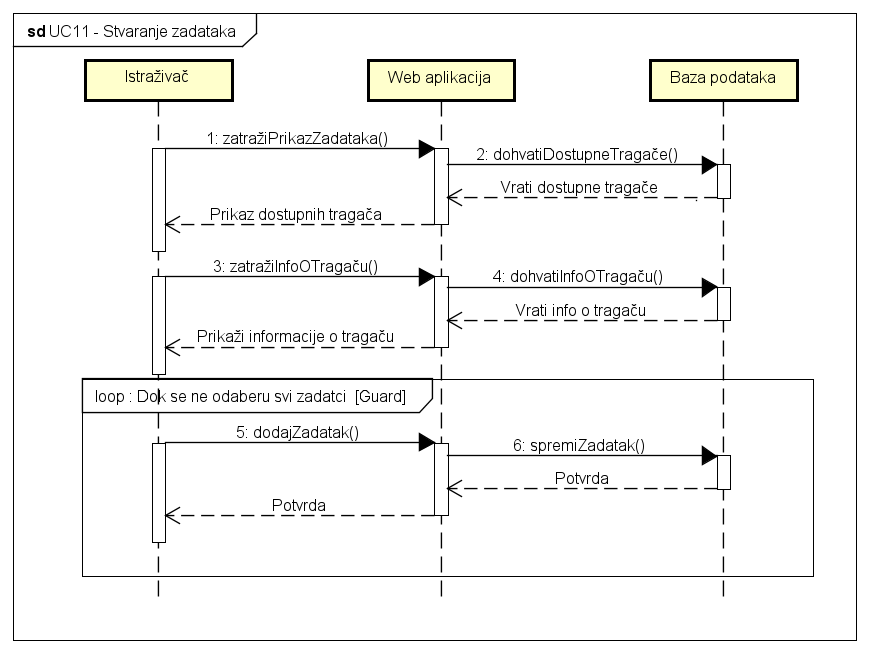
\includegraphics[scale=0.7]{slike/UC11_sekv.PNG} %veličina slike u odnosu na originalnu datoteku i pozicija slike
					\centering
					\caption{Sekvencijski dijagram - UC11}
					\label{fig:promjene}
				\end{figure}
				\eject
				
				\noindent \textbf{Obrazac uporabe UC15 - Prikaz karte za tragača}\\
				
				\noindent Tragač šalje zahtjev za prikazom stranice za odabir karte. Poslužitelj prima zahtjev, iz baze podataka dohvaća podatke o dostupnim akcijama te tragaču prikazuje stranicu na kojoj može odabrati kartu za određenu akciju te način prikaza informacija na karti (popis zadataka, trenutne pozicije ostalih tragača, trenutne pozicije životinja). Ako tragač odabere popis zadataka, prikazuju mu se njegovi zadaci te ih može pregledati i označiti odrađenim. Ako tragač odabere prikaz karte i trenutnih pozicija, poslužitelj prima zahtjev, dohvaća podatke o pozicijama iz baze podataka i tragaču šalje stranicu na kojoj se prikazuje karta sa svim traženim pozicijama.
				
				\begin{figure}[H]
					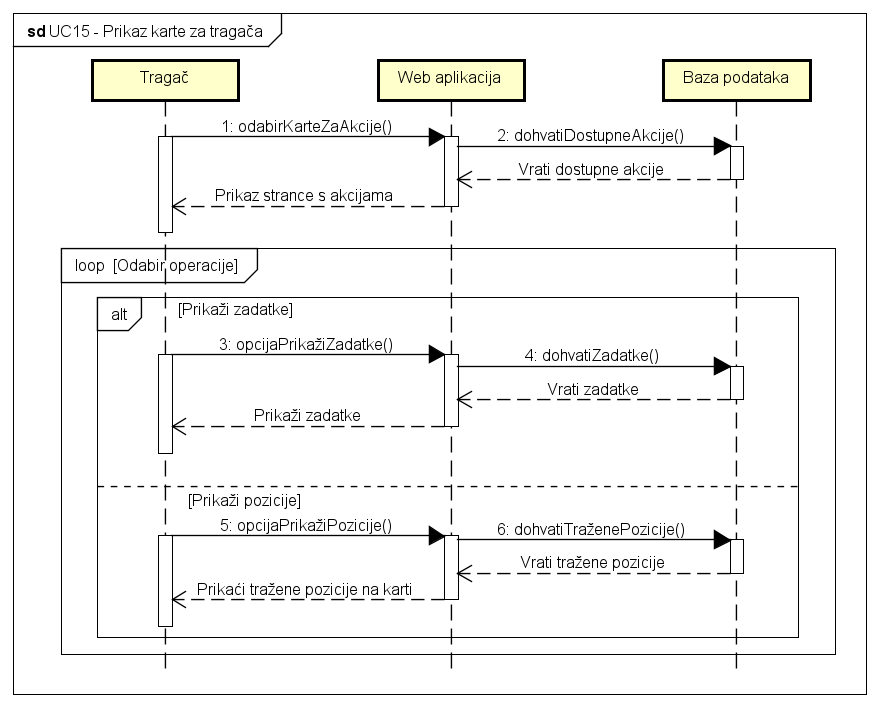
\includegraphics[scale=0.7]{slike/UC15_sekv.PNG} %veličina slike u odnosu na originalnu datoteku i pozicija slike
					\centering
					\caption{Sekvencijski dijagram - UC15}
					\label{fig:promjene}
				\end{figure}
	
		\section{Ostali zahtjevi}
		
			 
			 \begin{packed_item}
			 	\item Vrijeme odziva poslužitelja mora biti maksimalno 10 sekundi.
			 	\item Ne smiju postojati neautorizirane naredbe od strane registriranih korisnika.
			 	\item Neregistrirani korisnici ne smiju imati pristup informacijama akcija i karata.
			 	\item Aplikacija treba podržavati hrvatsku abecedu.
			 	\item Neplanirano korištenje korisničkog sučelja ne smije narušiti sigurnost podataka.
			 	\item Aplikacija treba biti responzivna.
			 	\item Pregledna i lagana navigacija po aplikaciji.
			 	\item Prikaz se mora jednostavno i intuitivno prilagoditi veličini zaslona.
			 	\item Aplikacija ne smije preopteretiti radnu memoriju.
			 	\item Lozinka registriranog korisnika u bazi podataka treba biti kriptirana.
			 	\item Komunikacija s bazom podataka treba biti kvalitetno zaštićena.
			 	\item Aplikaciju treba moći koristiti više korisnika istovremeno bez poteškoća.
			 \end{packed_item}
			 
			 
			 
	